\chapter{Systematic Design of Optimal Low-Thrust Transfers for the Three-Body Problem}
\section{Introduction}
Spacecraft and space systems serve a critical role in understanding and enabling modern life.
The Global Positioning System (GPS) and many scientific instruments such as the Hubble Space Telescope, Voyager missions, and the recent Rosetta mission have expanded our understanding of the universe.
Designing spacecraft trajectories is a classic and ongoing topic of research.
With the addition of propulsion devices spacecraft are capable of departing from the free motion trajectory.
Much previous work is based on an impulsive thrust assumption which allows for instantaneous changes in spacecraft velocity.
This assumption does not allow for the analysis of many low thrust propulsion devices which must operate over extended periods of time.
Electric propulsion offers higher specific impulse and much greater efficiencies than traditional chemical propulsion.

Minimizing fuel used on board spacecraft is vital to maximizing mission life and esuring continued access to vital space capabilities.
The low energy maneuvers typical of electric propulsion require increased thrust intervals where propogation and dynamic errors must be minimized.
Incorporation of higher fidelity dynamic models and improved integration methods allow for accurate and efficient computation of spacecraft trajectories.
In this work, the dynamics of a controlled spacecraft in the Circular Restricted Three Body(CRTBP) system are developed.
An optimal control formulation is developed which combines the concept of reachability and return, or Poincar\'e, maps to allow design of transfers.

This work is divided into the following sections.
A description of the three-body problem and several important properties are provided in Section~\ref{sec:crtbp}.
The concepts of Poincar\'e sections and invariant manifolds from dynamical systems theory are introduced and applied to the current work in Section~\ref{sec:dst}.
An indirect optimal control problem is formulated in Section~\ref{sec:opt} which combines the concepts of state reachability and Poincar\'e sections.
A numerical example illustrating the use of the proposed method is presented.

\section{Equations of Motion}\label{sec:crtbp}
Throughout history, scholars have sought to describe the motion of the planets and heavenly bodies of our solar system.
In his pivotal work~\cite{newton1999} Isaac Newton supplied a mathematical model for the astronomical observations of his predecessors.
Newton's Law of Universal Gravitation provides a physical and mathematical basis for the motion of point masses under the influence of gravity. 
The model for universal gravitation is expressed as
\begin{equation}
	F_g = - \frac{G m_1 m_2}{\norm{r_{12}^3}} r_{12}
	\label{eq:universal_gravitation}
\end{equation}
where \( F_g\) is the gravitational force of point mass \(m_1\) acting upon mass \( m_2\).
The relative position vector \( r_{12} \) is directed from \( m_1\) to \(m_2\) and \( G\) is the universal gravitational constant.
Combining~\eqref{eq:universal_gravitation} with Newton's second law allows us to expand this model to include the mutual attraction of \( N \) point masses on the particle of interest
\begin{equation}
	m_i \ddot{r_i} = -G \sum_{\substack{j=1 \\ j\neq i}}^n \frac{m_i m_j}{\norm{r_{ji}^3}} r_{ji}
	\label{eq:n_body}
\end{equation}
The vector \( r_i \in \R^{3\times1}\) is position of the particle of interest with respect to an inertially fixed observer and the vectors \( r_{ji} = r_i - r_j \) define the relative displacement of the \( j\textsuperscript{th}\) body with respect to the particle of interest.

In general, there is no closed-form analytical solution to~\eqref{eq:n_body}.
However, in the case that the system is reduced to only two bodies the relative motion is defined by conic sections and a complete solution is known~\cite{bate1971}.
In many mission scenarios, this two-body (Keplerain) solution is valid and has been applied successfully~\cite{vallado2001}.
Many implementations treat the effects of multiple gravitational bodies and higher order gravitational harmonics as perturbations to the two-body model. 
However, situations exists where additional gravitational influences must be directly modeled.
The addition of multiple attractive bodies afford solutions that only emerge in these higher order representations.

\subsection{Planar Circular Restricted Three Body Problem}
The model for the equations of motion is focused on N = 3 bodies reducing~\eqref{eq:n_body} to three particles and defining particle \(P_3\) as the body of interest leaves
\begin{equation}
	m_3\ddot{r_3} = -G \frac{m_1 m_3}{\norm{r_{13}}^3} r_{13} - G \frac{m_1 m_2}{\norm{r_{23}}^3} r_{23}
	\label{eq:threebody}
\end{equation}
In order to solve~\eqref{eq:threebody} analytically the motion of \( P_1 \) and \( P_2\) must be known a priori. 
Without this time history of \( r_1\) and \( r_2\) the equations of motion of all three bodies must be evaluated simultaneously. 
This results in 18 scalar first-order differential equations requiring 18 integrals of motion for a complete solution.
Unfortunately, only ten integrals of motion are known: six from conservation of system linear momentum, three from the conservation of system angular momentum, and one from the conservation of system energy.
However, several simplifying assumptions produce valuable insight without the loss of significant fidelity~\cite{szebehely1967}.

The first simplification assumes that the mass of \( P_3\) is negligible when compared to the masses of the other two bodies.
As a result, the motion of the much more massive \(P_1\) and \(P_2\), termed primaries, is unaffected by the motion of \(P_3\).
For example, the masses \(P_1\) and \(P_2\) could represent the Earth-Moon system while the particle \(P_3\) represents the motion of a spacecraft.
Since the motion of the primaries is no longer dependent on \(P_3\) they are represented as a two-body system with known conic solution.
For most systems of interest this is a closed conic section and is further simplified to circular orbits about their common barycenter.
A final assumption constrains the motion of \(P_3\) to the orbital plane defined by the primaries. 
This planar assumption reduces the complexity of the following developments yet allows for the modeling of a wide variety of typically encountered scenarios.

The differential equation in~\eqref{eq:threebody} represents the motion of \(P_3\) relative to an inertial observer.
However, expressing the dynamics in a rotating reference frame offers much greater insight into the system structure. 
The inertial frame is defined by the orthogonal unit vectors \(X-Y-Z\) with the origin fixed to the common system barycenter as shown in Figure~\ref{fig:rot_frame}.
The rotating frame is defined by the \(x,y, \text{ and } z \) vectors shown. 
The \(x\)-axis is directed along vector connecting the primaries and the \(y\) is orthogonal to it. 
The \(x-y\) rotates with respect to the inertial frame with a constant angular velocity equal to the mean motion.
\begin{figure}[htbp]%
\centering
        \begin{subfigure}[H]{0.5\columnwidth}%
                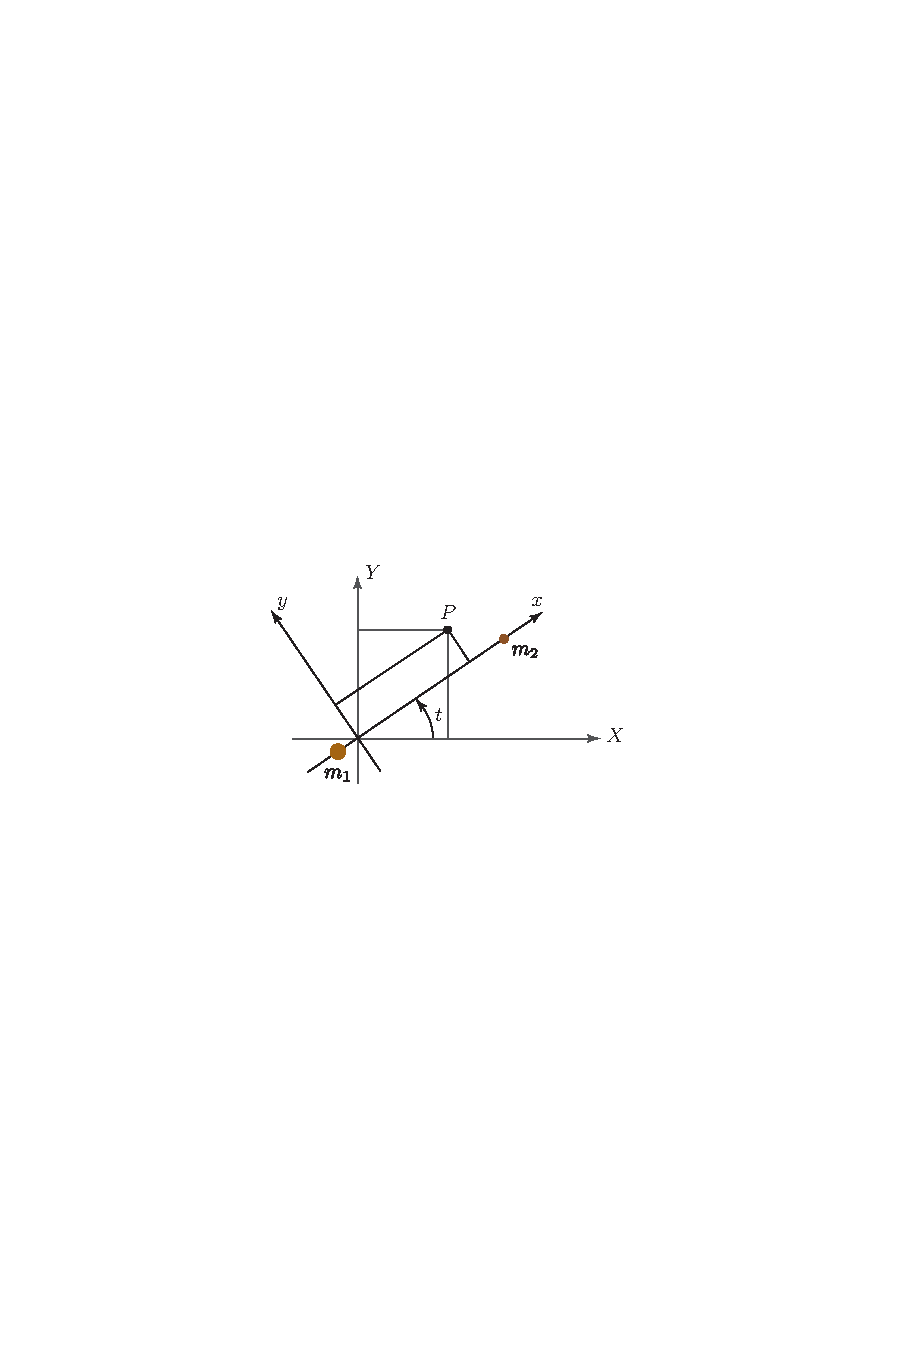
\includegraphics[width=\textwidth]{figures/2015_SSPI/rot_frame}%
                \caption{Inertial and rotating frames}%
                \label{fig:rot_frame}%
        \end{subfigure}%
        ~
        \begin{subfigure}[H]{0.5\columnwidth}%
                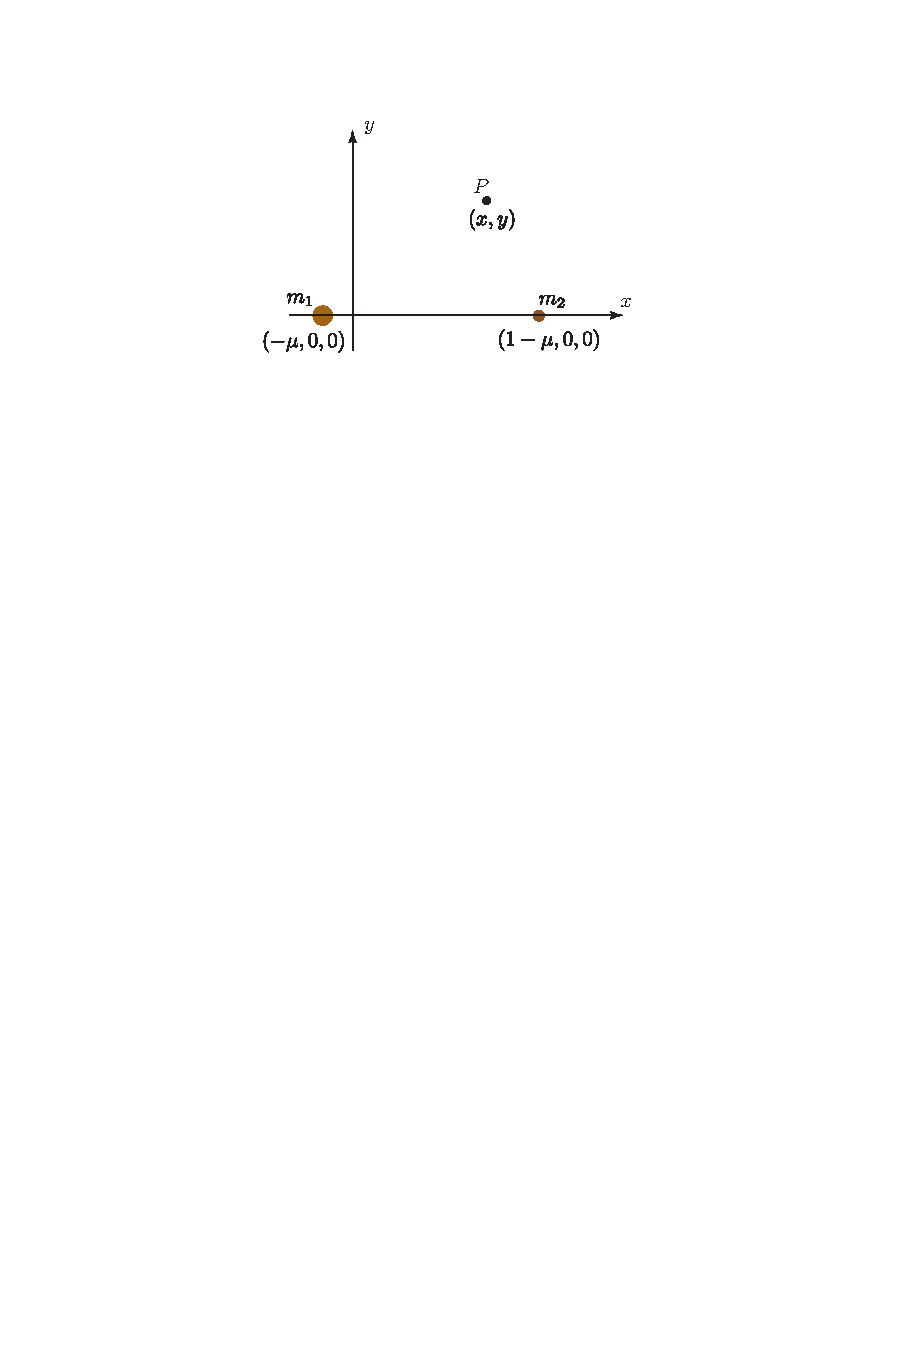
\includegraphics[width=\textwidth]{figures/2015_SSPI/rot_frame_def}%
                \caption{Rotating Coordinate System}%
                \label{fig:rot_frame_def}%
        \end{subfigure}%
		\label{fig:ref_frame}%
\end{figure}%
In following the typical formulation the system is also made nondimensional by the appropriate choice of the characteristic mass, length, and time.
A variety of typical values is provided by~\cite{koon2000}.
As a result, the system can be characterized by a single mass parameter \( \mu \).
\begin{equation}
	\mu = \frac{m_2}{m_1+m_2}
	\label{eq:mass_param}
\end{equation}
With~\eqref{eq:mass_param} the larger primary, \(m_1\) by convention, is located at \( \left(  -\mu , 0 , 0\right)\) and the smaller \( m_2\) is located at \( \left( 1-\mu , 0 , 0\right)\).
In the rotating frame the Lagrangian is given by
\begin{equation}
	L = \frac{1}{2} \left( \left( \dot{x} -y \right)^2 + \left( \dot{y} + y \right)^2 \right) + \frac{1-\mu}{r_1} + \frac{\mu}{r_2}
	\label{eq:lagrangian}
\end{equation}
where the distance \(r_1\) and \(r_2\) of the spacecraft to each primary is defined in rotating coordinates as
\begin{align}
	r_1 &= \sqrt{\left( x+ \mu\right)^2 + y^2} \\
	r_2 &= \sqrt{\left( x - 1 + \mu\right)^2 + y^2}
	\label{eq:distances}
\end{align}
Application of the Euler-Lagrange equations results in following equations of motion defined in the rotating reference frame
\begin{align}
	\ddot{x} - 2 \dot{y} + \frac{\partial}{\partial x} U &= u_x \nonumber \\
	\ddot{y} + 2 \dot{y} + \frac{\partial}{\partial y} U &= u_y 
	\label{eq:cont_eom}
\end{align}
where the effective potential \( U\) is defined as
\begin{equation}
	U = \frac{1}{2} \left( x^2 y^2\right) + \frac{1-\mu}{r_1} + \frac{\mu}{r_2}
	\label{eq:eff_pot}
\end{equation}
and the control inputs are defined as \( u_x\) and \(u_y\).
Defining the state \( \bar{x} = \begin{bmatrix}\bar{r} &\bar{v} \end{bmatrix}\) with \(\bar{r} \in \R^{2\times1}\) and \(\bar{v} \in \R^{2\times1}\) representing the position and velocity with respect to the system barycenter, respectively.
The equations of motion may be rewritten in state space form
\begin{equation}
	\left[\begin{array}{c} \dot{\bar{r}} \\ \dot{\bar{v}} \end{array} \right] = 
	\left[ \begin{array}{c} \bar{v} \\ A \bar{v} + \nabla U + \bar{u}(t) \end{array} \right] = f\left( t,x, u\right)
\end{equation}
where the matrix \( A \) and psuedo gravitational potential gradient \( \nabla U\) are
\begin{equation}\label{eq:A_mat}
	A = \left[ \begin{array}{ccc} 0 & 2 & 0 \\ -2 & 0 & 0 \\ 0 & 0 & 0 \end{array} \right]
\end{equation}
\begin{equation} \label{eq:grav_pot}
	\nabla U = \left[ \begin{array}{c} x - \frac{ \left(1 - \mu\right) \left(x + \mu\right)}{r_1^3} - \frac{\mu \left( x+ \mu -1\right)}{r_2^3} \\
											y - \frac{ \left(1 - \mu\right) y}{r_1^3} - \frac{\mu y}{r_2^3} \\
											- \frac{ \left(1 - \mu\right) z}{r_1^3} - \frac{\mu z}{r_2^3}\end{array}\right]
					= \left[\begin{array}{c} U_x \\ U_y \\ U_z\end{array} \right]
\end{equation}
A comprehensive development of these equations of motion and related properties is provided by~\cite{szebehely1967}.
\subsection{Integral of motion}
There exists a single integral, or constant of motion for the three-body problem~\cite{lanczos1970,szebehely1967}.
This energy constant is analogous to the total mechanical energy, however is a non physical quantity arising from the problem formulation~\cite{szebehely1967}.
Also known as the Jacobi constant, it is defined as a function of the position and velocity in the rotating frame
\begin{equation}
	E\left( \bar{r} , \bar{v} \right) = \frac{1}{2}\left( \dot{x}^2 + \dot{y}^2\right) - U\left(x,y \right)
	\label{eq:jacobi}
\end{equation}
The Jacobi integral~\eqref{eq:jacobi} divides the phase space into distinct regions based on the energy level of the body of interest.
Fixing the Jacobi integral to a constant defines zero velocity curves, which are the locus of points where the kinetic energy, and hence velocity vanishes.
As seen in Figure~\ref{fig:energy_contour}, the phase space is divided into distinct realms based on the energy level.
\begin{figure}[htbp]
	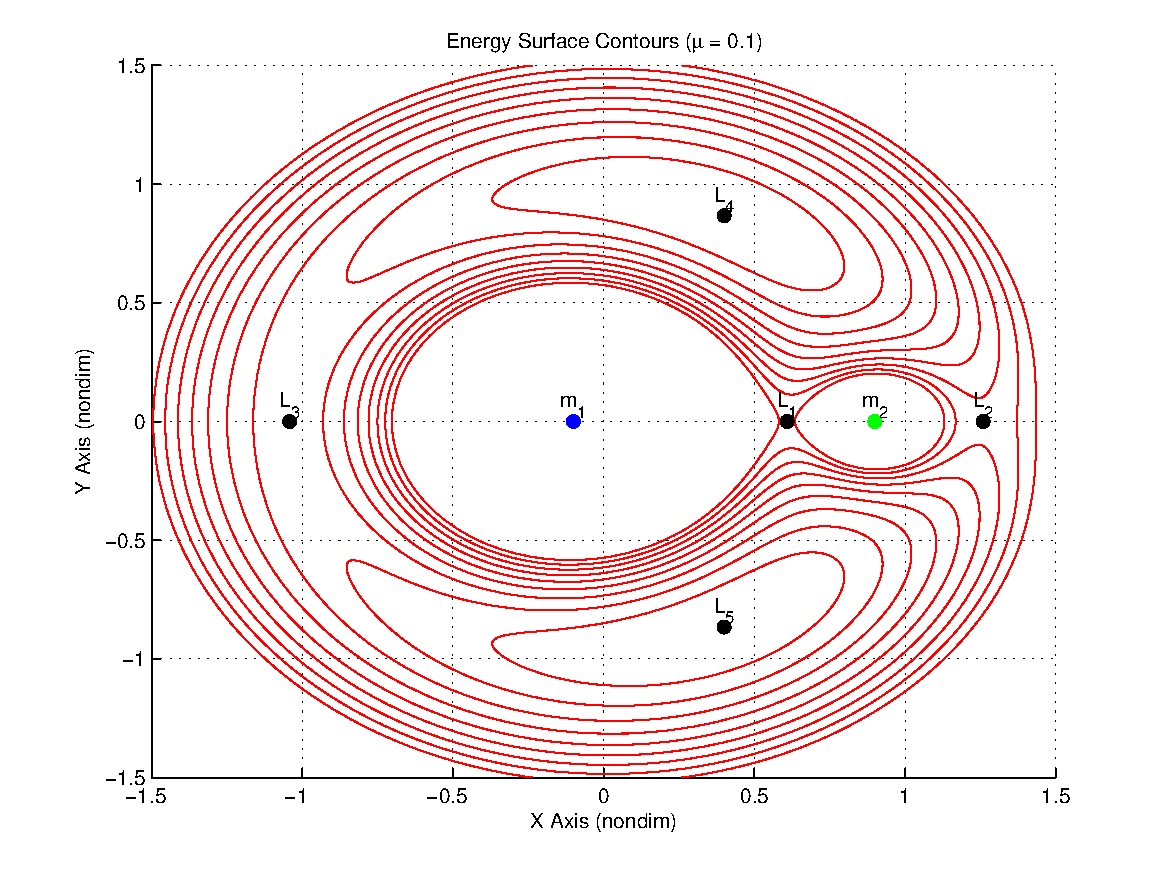
\includegraphics[width=\textwidth]{figures/2015_SSPI/energy_contours}
	\caption{Contour Plot of Jacobi Integral}
	\label{fig:energy_contour}
\end{figure} 
In the vicinity of \( m_1\) or \(m_2\) we have a potential well. 
As the energy level increases we find that there are five critical points of the effective potential~\eqref{eq:eff_pot} where the slope is zero.
Three collinear saddle points on the \(x\) axis and two symmetric points off the \(x\) axis.
These equilibrium, or Lagrange points, are labeled \( L_i, i = 1, \hdots, 5 \) and are shown in Figure~\ref{fig:energy_contour}.

The stability in the vicinity of the Lagrange points is determined through use of a local linear approximation 
\begin{equation}
	A = \frac{\partial f}{\partial \bar{x}}
	\label{eq:jacobian}
\end{equation}
The local stability of each Lagrange point can be classified in the sense of Lyapunov through analysis of the eigenvalues, \( \lambda_i \) of~\eqref{eq:jacobian}.
\begin{itemize}
	\item if \(\Real{\lambda_i} < 0 \, \forall \, i\) the equilibrium point is stable in the nonlinear system
	\item if \(\Real{\lambda_i} > 0  \text{ for any } i\) the equilibrium point is unstable in the nonlinear system
	\item if \(\Real{\lambda_i} = 0 \text{ for some } i \text { and } \Real{\lambda_i} < 0 \) the equilibrium point is marginally stable and the nonlinear stability properties must be determined through other means
\end{itemize}
In general, the motion near an equilibrium point will exhibit a combination of decaying, growing, and oscillatory components. 
For example, in the Earth-Moon system the collinear Lagrange points, \(L_1\), \(L_2\), and \( L_3\) exhibit all three behaviors while the \(L_4\) and \(L_5\) points exhibit purely oscillatory behavior and higher order methods are required to determine stability.
\section{Periodic Orbits}\label{sec:dst}
Infinite number of periodic orbits exist in the vicinity of the Lagrange points of the three-body problem.
As a result, one must apply numerical techniques in order to determine and calculate their precise locations.
Following the work of~\cite{howell1994,connor-howell1984a} a differential corrections procedure is developed to target specific periodic planar Lyapunov orbits.
For planar periodic orbits, it is desired to determine perpendicular \(x\)-axis crossings with a specific value.
After one half period, a candidate orbit should again make a perpendicular crossing of the form \( \bar{x} = \left[\begin{array}{cccc} x & 0 & 0 & \dot{y} \end{array}\right]\).
Since solutions of the three body problem are symmetric about the \(x\)-axis we are only required to numerically integrate half of the periodic orbit.

In this iterative procedure, a mapping is required that relates variations of the final target state to variations of the initial state.
The State Transition Matrix serves to linearly transform variations of the initial state at \( t_0\) to those variations at time \(t\)~\cite{slotine1991}.
\begin{equation}
	\delta x(t) = \frac{\partial \bar{x}}{\partial \bar{x}_0} \delta \bar{x}_0 = \Phi(t,t_0) \delta \bar{x}_0
	\label{eq:variational_state}
\end{equation}
The matrix derivative in~\eqref{eq:variational_state} is computed in a similar manner as that of~\eqref{eq:jacobian} and is governed by the differential equation
\begin{equation}
	\dot{\Phi}(t,t_0) = \frac{\partial f(x, u , t)}{\partial \bar{x}(t)} \Phi(t,t_0) = A(t) \Phi(t,t_0)
	\label{eq:stm}
\end{equation}
Given a system of \(n\) state equations, the State Transition Matrix requires propagation of an additional \(n^2\) differential equations. 
Significant computational advantages can be realized in the case of linear time invariant systems.

An update equation can be determined that relates variations of the target state after one half period \(t_1 = \frac{T}{2} \) to the initial state
\begin{equation}
	\begin{bmatrix}
		\delta x_1 \\ 0 \\ \delta \dot{x_1} \\ \delta \dot{y_1}
	\end{bmatrix}
	=
	\begin{bmatrix}
		\Phi_{11} & \Phi_{14} \\
		\Phi_{21} & \Phi_{24} \\
		\Phi_{31} & \Phi_{34} \\
		\Phi_{41} & \Phi_{44} \\
	\end{bmatrix}
	- \frac{1}{\dot{y_1}}
	\begin{bmatrix}
		\dot{x_1} \\ \dot{y_1} \\ \ddot{x_1} \\ \ddot{y_1}
	\end{bmatrix}
	\begin{bmatrix}
		\Phi_{21} & \Phi_{24}
	\end{bmatrix}	
	\begin{bmatrix}
		\delta x_0 \\ \delta \dot{y_0}
	\end{bmatrix}
	\label{eq:diff_corr}
\end{equation}
Two update equations can be determined by inverting~\eqref{eq:diff_corr} which either hold \(x(0)\) or \(\dot{y}(0)\).
In an iterative procedure, planar periodic orbits are determined for a specified Jacobi energy value about the Earth-Moon \(L_1\) and \( L_2\) Lagrange points.
Families of periodic orbits are generated through a numerical continuation process as illustrated in Figure~\ref{fig:periodic_family}.
\begin{figure}
	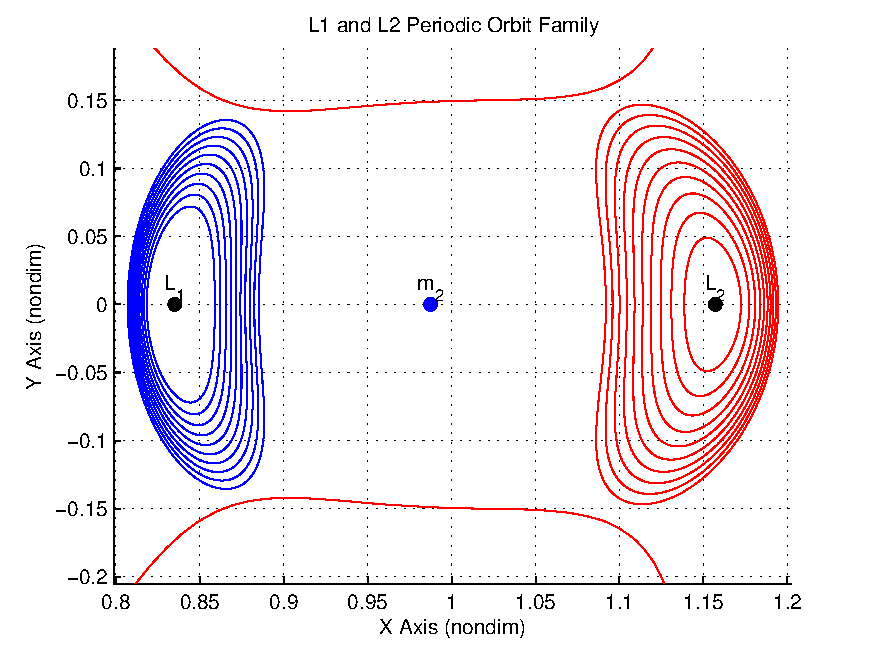
\includegraphics[width = \textwidth]{figures/2015_SSPI/L1L2_periodic_family}
	\caption{Family of Periodic Orbits\label{fig:periodic_family}}
\end{figure}
This process is readily extended to the spatial three-body problem and many other classes of periodic orbits have been investigated~\cite{mains1993,connor-howell1984a,breakwell1979,richardson1980}.
\subsection{Invariant Manifolds and Poincar\'e section}
As described previously in Section~\ref{sec:dst} the Jacobian~\eqref{eq:jacobian} can be used to approximate the local stability properties of a solution.
To a first order approximation, a solution that starts from a perturbed initial state \( \bar{x}_0 + \delta \bar{x}_0 \) will after one period \(T\) be displaced by
\begin{equation}
	\delta \bar{x}(T) = \Phi(T,0) \delta \bar{x}_0 = M \delta \bar{x}_0
	\label{eq:monodromy}
\end{equation}
where the matrix, \(M\), is defined as the monodromy matrix of the period orbit, which determines the growth or decay of initial perturbations from the periodic orbit.
After a periodic orbit is determined, the state transition matrix is numerically integrated from time \(0\) to \(T\) along the periodic orbit.
In order to reduce the computational burden of propagating the state transition matrix, the invariance of the three-body problem is used to redefine the monodromy matrix
\begin{equation}
	M = \Phi(T,0) = A \Phi\left(\frac{T}{2},0\right)^{-1} A \Phi\left(\frac{T}{2},0\right)
	\label{eq:monodromy_half}
\end{equation}
where the matrix \(A\) in~\eqref{eq:monodromy_half} is the linear transformation
\begin{equation*}
	A = \begin{bmatrix}
		1 & 0 & 0 & 0\\
		0 & -1 & 0 & 0 \\
		0 & 0 & -1 & 0 \\
		0 & 0 & 0 & 1
	\end{bmatrix}
\end{equation*}
Applying~\eqref{eq:monodromy_half} requires integration of the state transition matrix over a half period, drastically reducing the computational burden.
For the planar periodic orbit, the four eigenvalues of \(M\) are classified according to the local stability.
\begin{equation*}
	\lambda_1 > 1 \quad \lambda_2 = \frac{1}{\lambda_1} \quad \lambda_3 = \lambda_4 = 1
\end{equation*}
where \(\lambda_1\) is associated with the unstable direction while \(\lambda_2\) is associated with the stable direction.
The corresponding eigenvectors are used to approximate the local invariant manifold.
A perturbation in the direction of the stable or unstable eigenvector is used to generate initial conditions for the manifolds.
\begin{align}
	X^s(X_0) &= X_0 \pm \epsilon Y^s(X_0) \nonumber \\
	X^u(X_0) &= X_0 \pm \epsilon Y^u(X_0)
	\label{eq:manifold_initial}
\end{align}
where the vectors \(Y^s \text{ and } Y^u \) are the normalized eigenvectors associated with the stable and unstable eigenvalues, respectively.
In~\eqref{eq:manifold_initial}, \( \epsilon \) is a small displacement from the periodic orbit. 
Numerically integrating these initial conditions over the entire periodic allows for globalization of the invariant manifolds.
The parameter \(\epsilon\) should be small enough to be within the validity of the linear approximation yet not too small such that the time of flight of the manifold grows too large.
\begin{figure}
     \centering
        \begin{subfigure}[b]{0.5\textwidth}
                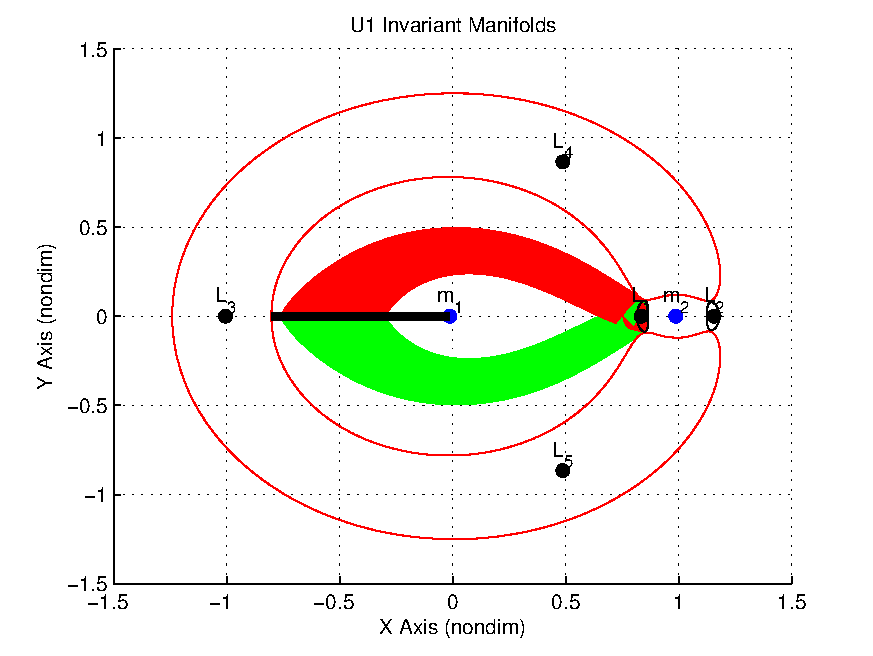
\includegraphics[width=\columnwidth]{figures/2015_SSPI/U1_Manifolds}
                \caption{U1 Manifolds}
                \label{fig:u1_manifolds}
        \end{subfigure}%
        ~%add desired spacing between images, e. g. ~, \quad, \qquad, \hfill etc.
          %(or a blank line to force the subfigure onto a new line)
        \begin{subfigure}[b]{0.5\textwidth}
                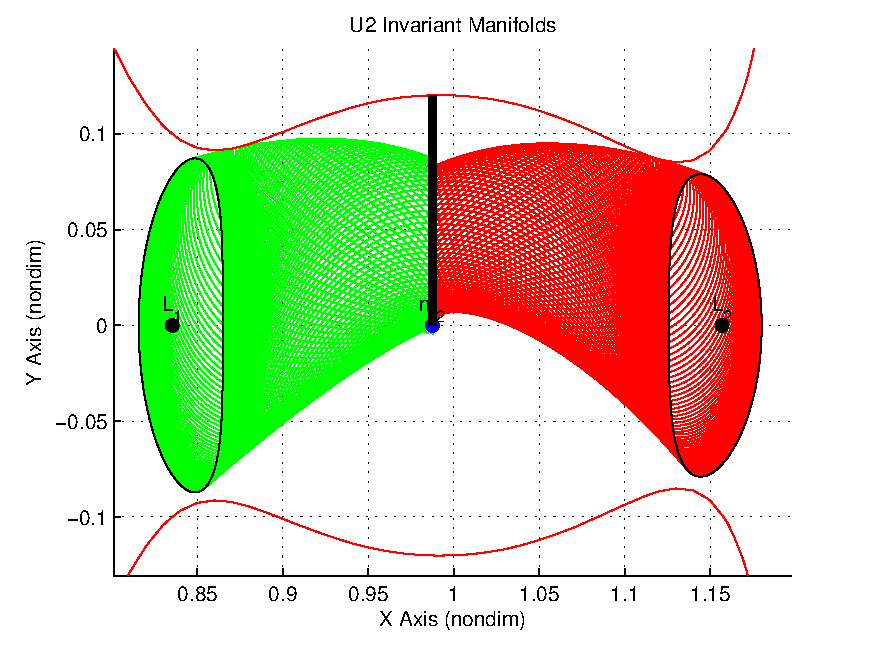
\includegraphics[width=\columnwidth]{figures/2015_SSPI/U2_Manifolds}
                \caption{U2 Manifolds}
                \label{fig:u2_manifolds}
        \end{subfigure}
        
        \begin{subfigure}[b]{0.5\textwidth}
                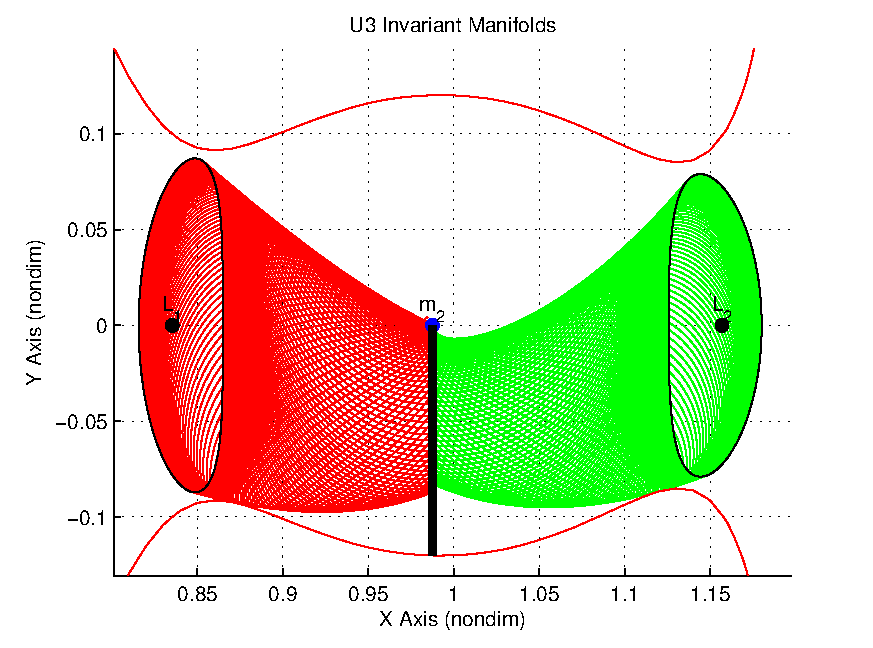
\includegraphics[width=\columnwidth]{figures/2015_SSPI/U3_Manifolds}
                \caption{U3 Manifolds}
                \label{fig:u3_manifolds}
        \end{subfigure}%
        ~%add desired spacing between images, e. g. ~, \quad, \qquad, \hfill etc.
          %(or a blank line to force the subfigure onto a new line)
        \begin{subfigure}[b]{0.5\textwidth}
                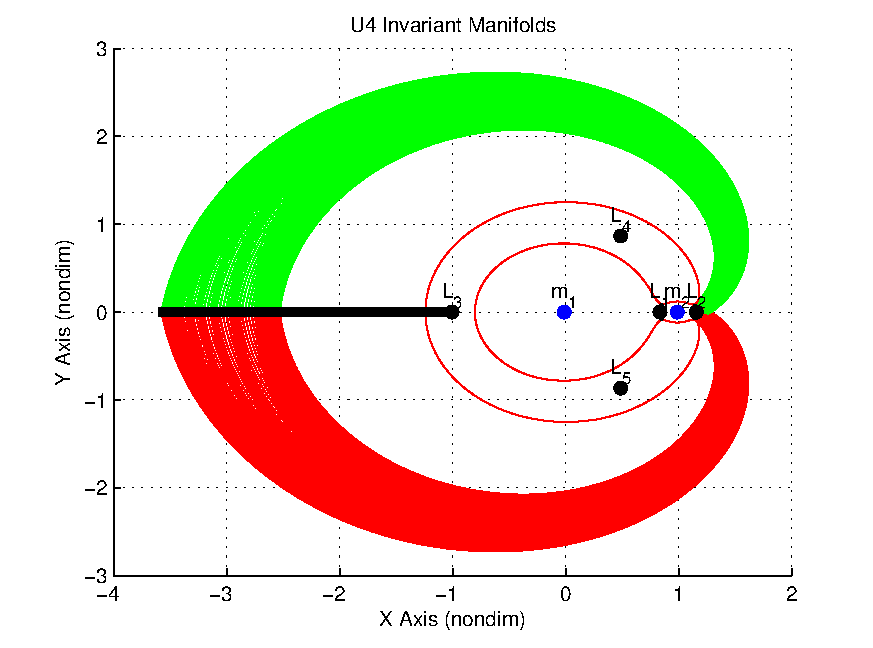
\includegraphics[width=\columnwidth]{figures/2015_SSPI/U4_Manifolds}
                \caption{U4 Manifolds}
                \label{fig:u4_manifolds}
        \end{subfigure}
        \caption{Invariant Manifolds for Planar Earth-Moon three body system}
	\label{fig:invariant_manifolds}
\end{figure}
Figure~\ref{fig:invariant_manifolds} shows the stable (green) and unstable (red) invariant manifolds for two planar periodic orbits about the \(L_1\) and \(L_2\) Lagrange points. 
These invariant manifolds only exist as a result of the dynamic formulation of the three-body problem in a rotating reference frame. 
In addition, all trajectories in Figure~\ref{fig:invariant_manifolds} exist at the same Jacobi energy value. 
The energy level~\eqref{eq:jacobi} is chosen such that a neck, or opening, exists in the region surrounding \(m_2\).
In this way, it is possible to design trajectories that intersect the invariant manifolds and connect widely separated regions of the state space. 
This technique has been heavily investigated in~\cite{koon2000}, applied to operational missions in~\cite{koon1999}, and applied to potential multi-moon orbiter missions in~\cite{tanaka2011}.
In addition, much recent work has focused on potential return missions to the Moon as in~\cite{zanzottera2012,campagnola2012,mingotti2011,ozimek2010a,mingotti2009}.

Another useful technique in the analysis of the free motion of dynamical systems is that of Poincar\'e section.
For a fixed energy level and a fixed section, the Poinar\'e surface reduces the state space from four to two dimensional~\cite{koon2001} for the planar three-body problem.
This greatly eases the design process and allows for a simple planar visualization of the intersection plane.
The Poincar\'e sections are denoted in Figure~\ref{fig:invariant_manifolds} by solid black lines and are labeled \(U_i\) for \(i = 1,\hdots,4\).
The sections are carefully chosen according to~\cite{koon2000b} to exploit heteroclinic and homoclinic connections between the realms.
Plotting the intersection of the invariant manifolds of Figure~\ref{fig:invariant_manifolds} with the chosen transversal sections allow us to plot the respective Poincar\'e sections in Figure~\ref{fig:poincare_sections}.
\begin{figure}
        	\centering
        	\begin{subfigure}[b]{0.5\textwidth}
                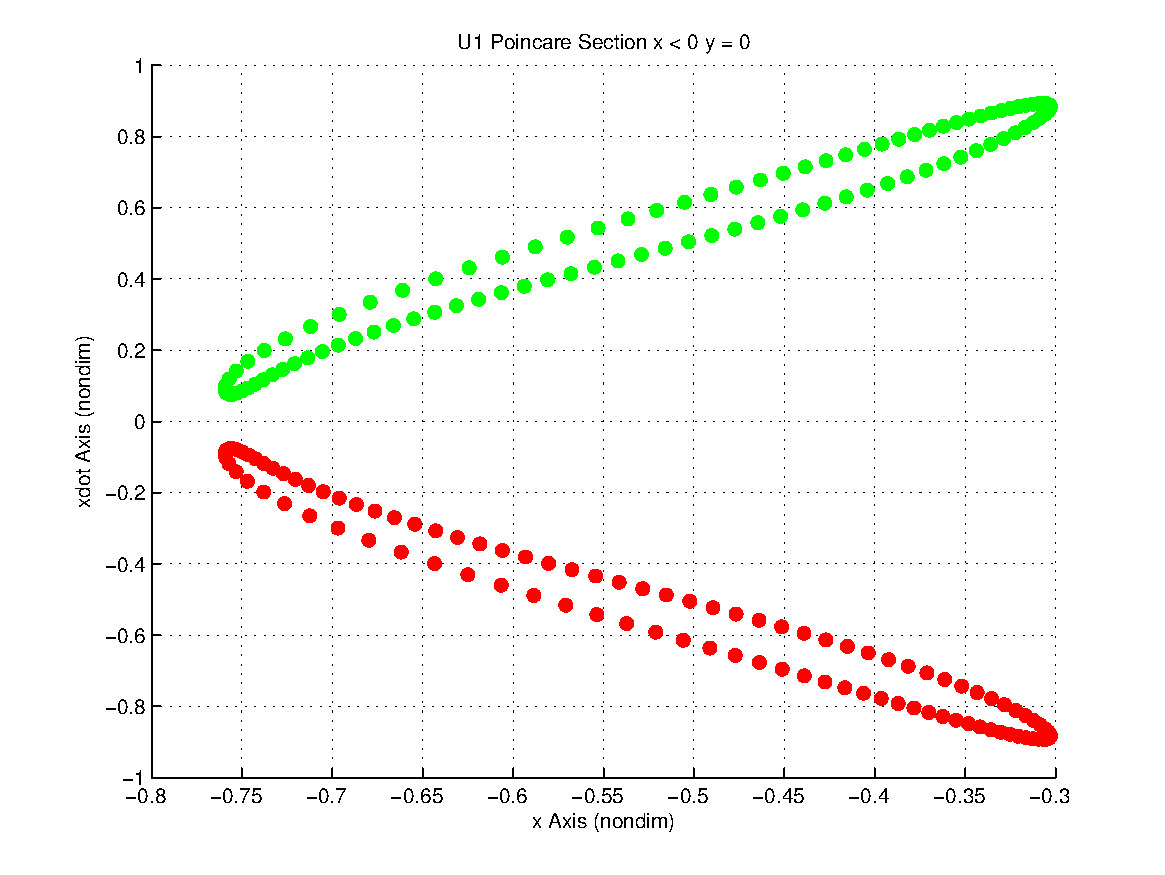
\includegraphics[width=\columnwidth]{figures/2015_SSPI/U1_poincare}
                \caption{U1 Poincar\'e}
                \label{fig:u1_poincare}
        	\end{subfigure}%
        	~%add desired spacing between images, e. g. ~, \quad, \qquad, \hfill etc.
          	%(or a blank line to force the subfigure onto a new line)
        	\begin{subfigure}[b]{0.5\textwidth}
                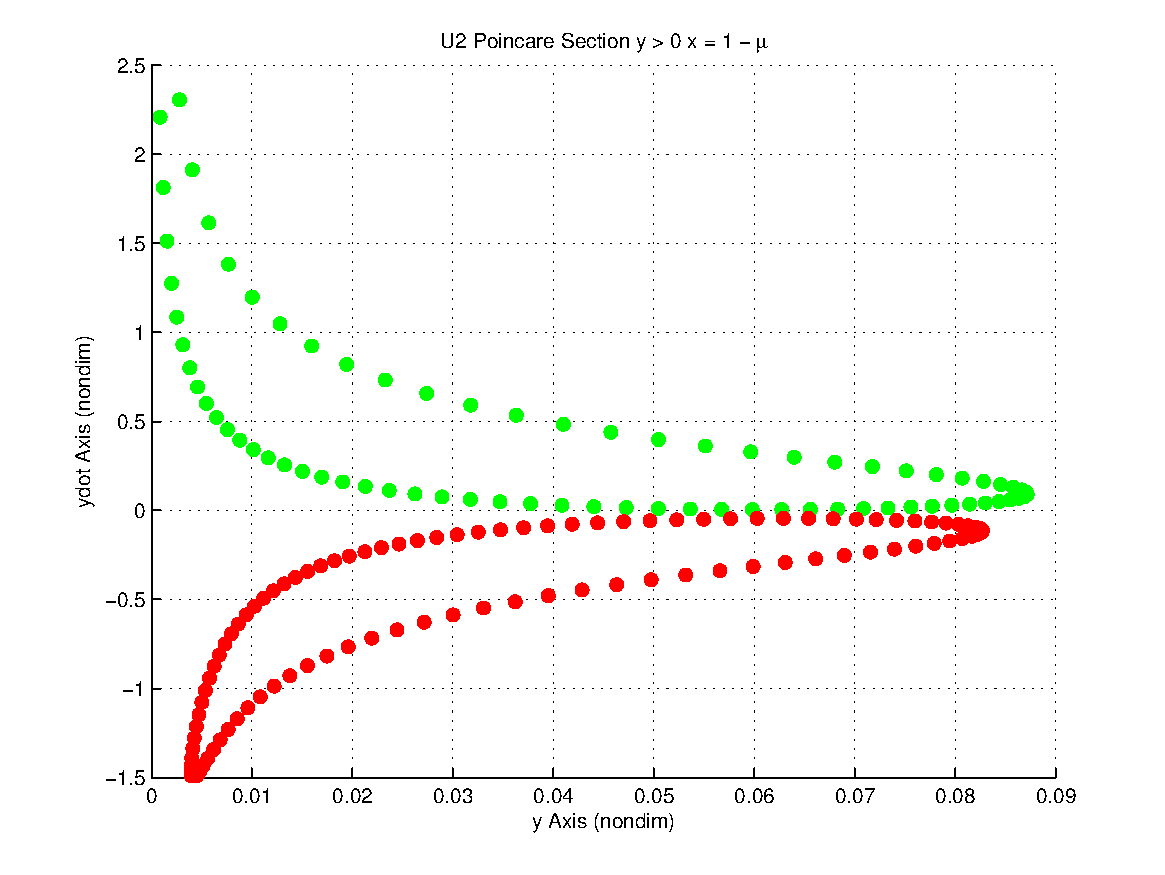
\includegraphics[width=\columnwidth]{figures/2015_SSPI/U2_poincare}
                \caption{U2 Poincar\'e}
                \label{fig:u2_poincare}
        	\end{subfigure}
        	
        	\begin{subfigure}[b]{0.5\textwidth}
                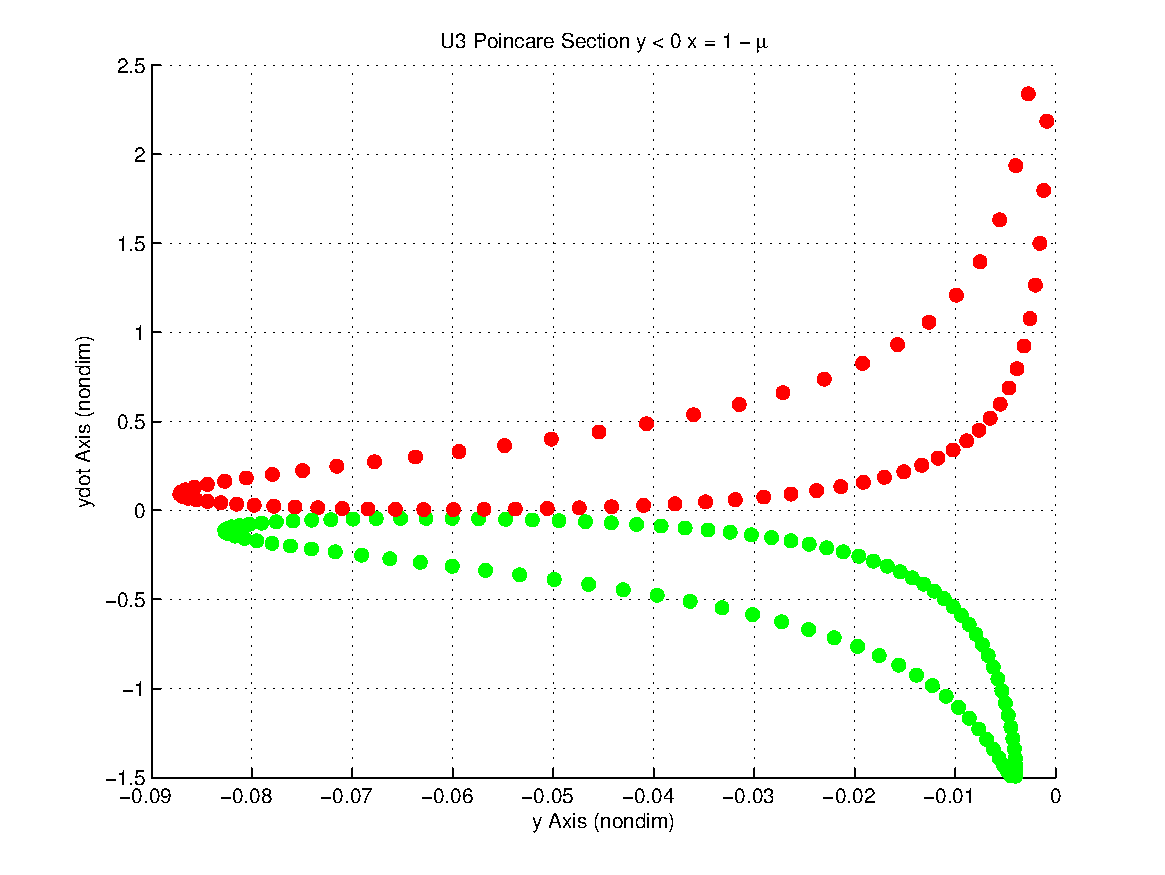
\includegraphics[width=\columnwidth]{figures/2015_SSPI/U3_poincare}
                \caption{U3 Poincar\'e}
                \label{fig:u3_poincare}
        	\end{subfigure}%
        	~%add desired spacing between images, e. g. ~, \quad, \qquad, \hfill etc.
          	%(or a blank line to force the subfigure onto a new line)
        	\begin{subfigure}[b]{0.5\textwidth}
        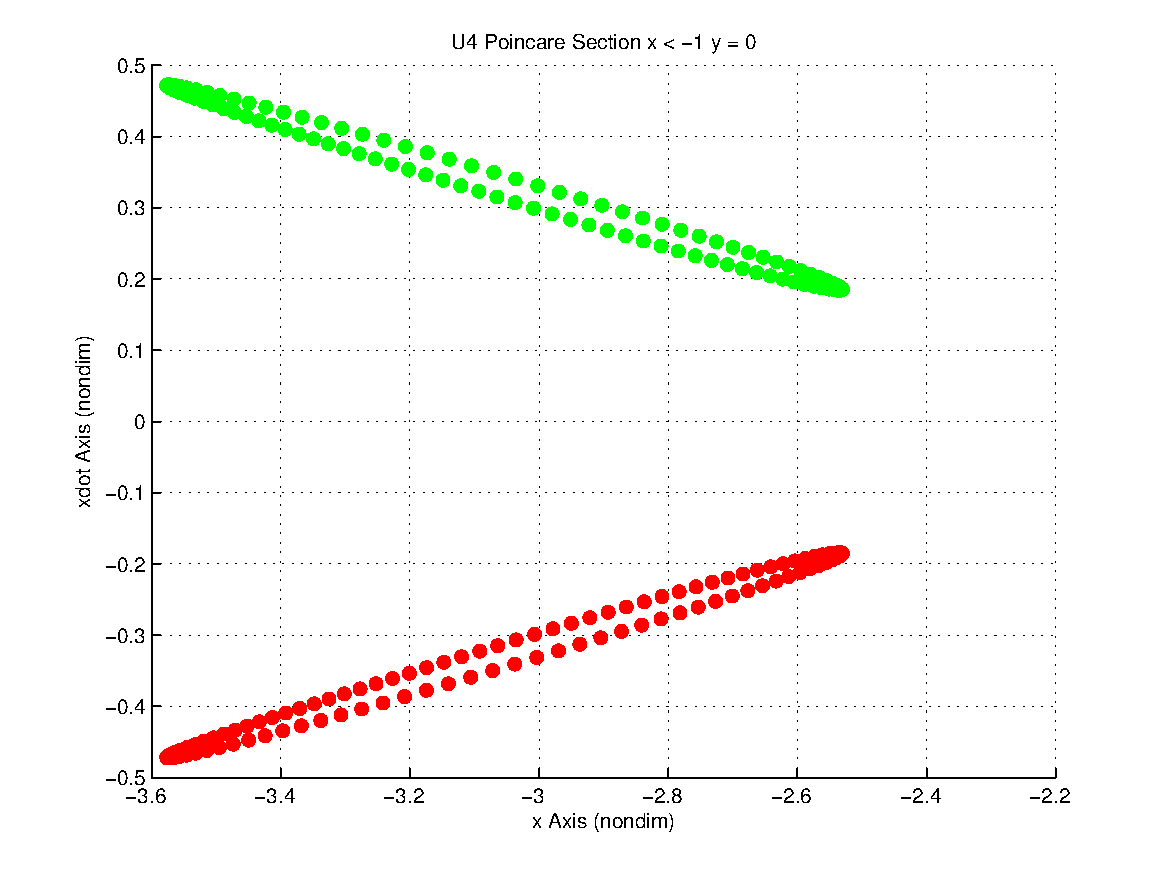
\includegraphics[width=\columnwidth]{figures/2015_SSPI/U4_poincare}
    	\caption{U4 Poincar\'e}
    	\label{fig:u4_poincare}
    \end{subfigure}
	\caption{Poincar\'e Sections for the Planar Earth-Moon three-body system}
	\label{fig:poincare_sections}
\end{figure}
Figures~\ref{fig:u4_poincare} and~\ref{fig:u1_poincare} show that the invariant manifolds do not intersect in this lower dimensional view. 
A control input is required to link the trajectories at this point and in previous work this thrust is assumed impulsive, or imparting an instantaneous change in velocity. 
This assumption is valid for large spacecraft capable of supporting high-thrust propulsion devices such as chemical rocket systems.
However, this assumption breaks down for low-thrust devices, such as electric propulsion, which have become more common on many recent cubesat missions and require extended thrusting durations in order to impart the necessary momentum change.
The following section will formulate and investigate a method to develop and analyze these low-thrust devices.
\section{Optimal Control}\label{sec:opt}
Optimal control theory has been widely applied to spacecraft trajectory design problems~\cite{peng2014,yue2009}.
Indirect optimal control allows for the calculation of state and control histories that minimize a cost functional. 
The concept of reachable sets has also seen widespread interest in the optimal control and system verifications communities. 
Given an initial condition and fixed horizon, the reachable set is the set of states attainable subject to the control constraints, which is closely related to optimal control theory~\cite{lygeros2004,lygeros2002,mitchell2002}.
In addition, the concept of reachability has also been more recently applied to the space domain~\cite{holzinger2012,holzinger2011,komendera2012a}. 
In this work, we seek to combine the concepts of reachable states with that of the Poincar\'e section in order to design orbital transfers.

The cost function is defined as
\begin{equation}
	J = -\frac{1}{2} \left( \bar{x}(t_f) - \bar{x}_{n}(t_f)\right)^T 
	\left[
	\begin{array}{cccc}
		1 & 0& 0& 0 \\
		 0& 0& 0& 0\\
		 0 & 0 & 1 &0\\
		 0 & 0& 0& 0
	\end{array}
	\right]
	\left( \bar{x}(t_f) - \bar{x}_{n}(t_f)\right)
	\label{eq:cost}
\end{equation}
The term \( \bar{x}_n(t_f) \) is the final state of a control free trajectory while the term \( \bar{x}(t_f) \) is the final state under the influence of the control input.
In this fashion, the aim is to maximize the distance of the final state from that of no control trajectory. 
A chosen Poincar\'e section is defined through the use of appropriate terminal constraints
\begin{subequations}
\begin{align}
     m_1 &= 0 = \frac{y(t_f) - L_{1y}}{x(t_f) - L_{1x}} - \tan{\alpha_d} \\ 
    m_2&= 0 = \frac{\dot{x}(t_f) - \dot{x_n}(t_f) }{x(t_f) -x_n(t_f) } - \tan{\theta_d} \\
    m_3 &= \begin{cases}
    	-\dot{x}(t_f) &\leq 0 \quad \text{if } 0 \leq \theta_d \leq \pi \\
		\dot{x}(t_f) &\leq 0 \quad \text{if } \pi \leq \theta_d \leq 2 \pi
    \end{cases}  \\
	 0 &\geq\bar{u}^T \bar{u} - u_{max}^2 
\end{align}
    \label{eq:constraints}
\end{subequations}
where the angles \( \alpha_d\) and \( \theta_d\) define the Poincar\'e section and a specific direction upon the section, respectively. 
The goal is to determine the control input \( \bar{u}(t)\) such that the cost function~\eqref{eq:cost} is minimized subject to the state equations of motion~\eqref{eq:cont_eom} and constraints~\eqref{eq:constraints}.
Application of the Euler-Lagrange equations allows us to derive the necessary conditions for optimality~\cite{bryson1975}.
\begin{subequations}\label{eq:necc_cond}
\begin{align}
	\dot{\lambda}^T &= - \frac{\partial H}{\partial x} \\
	0 &=  \frac{\partial H}{\partial u} \\
	0 &= \left[\frac{\partial \phi}{\partial x} + \beta^T \frac{\partial m}{\partial x} - \lambda^T(t_f) \right]^T \delta x(t_f) + \left. \left[ H^* + \frac{\partial \phi}{\partial t} \right] \right|_{t_f} \delta t
\end{align}
\end{subequations}
where the Hamiltonian \(H\) is defined as
\begin{equation}
	H = \lambda_r^T \bar{v} + \lambda_v^T \begin{bmatrix}0 & 2\\-2 & 0 \end{bmatrix} \bar{v} + \lambda_v^T \begin{bmatrix} U_x \\ U_y \end{bmatrix} + \lambda_v^T \bar{u}
	\label{eq:hamiltonian_opt}
\end{equation}
and \(\lambda \in \R^{n \times 1}\) is the costate and \(\beta \in \R^{3 \times 1} \) are the additional Lagrange multipliers associated with the terminal constraints in~\eqref{eq:constraints}.
This indirect optimal control formulation leads to a two point boundary value problem with split boundary conditions. 
By sweeping the angle \( \theta_d \) one can approximate the reachable set on the Poincar\'e section subject to the bounded control input. 

A numerical test case is presented to demonstrate this process and generate preliminary results.
The goal is to determine a transfer trajectory between two planar periodic orbits of the Earth-Moon system. 
The initial and target orbits are depicted in Figure~\ref{fig:opt_reach_trajectory} as the black periodic orbits.
From the initial state, a series of optimal trajectories are generated which all intersect the desired Poincar\'e section.
The intersection of these trajectories with the Poincar\'e section is shown in Figure~\ref{fig:north_poincare_reach}.
The reachable set is discretely approximated as the area enclosed by the optimal trajectories.
As the target state does not lie within the reachable set, another iteration of the optimal control calculation must be performed. 
The location on the reachable surface which lies closest to the target state is used to generate the initial conditions for the next iteration.
A second, or southern, trajectory calculation once again generates an approximation of the reachable set as shown in Figure~\ref{fig:south_reach}.
In this iteration, that target state is enclosed within the reachable set. 
\Cref{fig:opt_reach_trajectory} illustrates the completed optimal transfer trajectory.
As the solution is composed of two distinct optimal solutions there exists a discontinuity at the switching point.
This discontinuity is most evident in the control history shown in \Cref{fig:opt_reach_control}.
More general transfers would require multiple applications of this reachability computation and additional Poincar\'e sections.
This recursive method allows one to enlarge the attainable states on the Poincar\'e section.
General transfers are possible by combining powered segments along the invariant manifolds.
\begin{figure}[htbp]
    \centering
    \begin{subfigure}[b]{0.49\textwidth}
        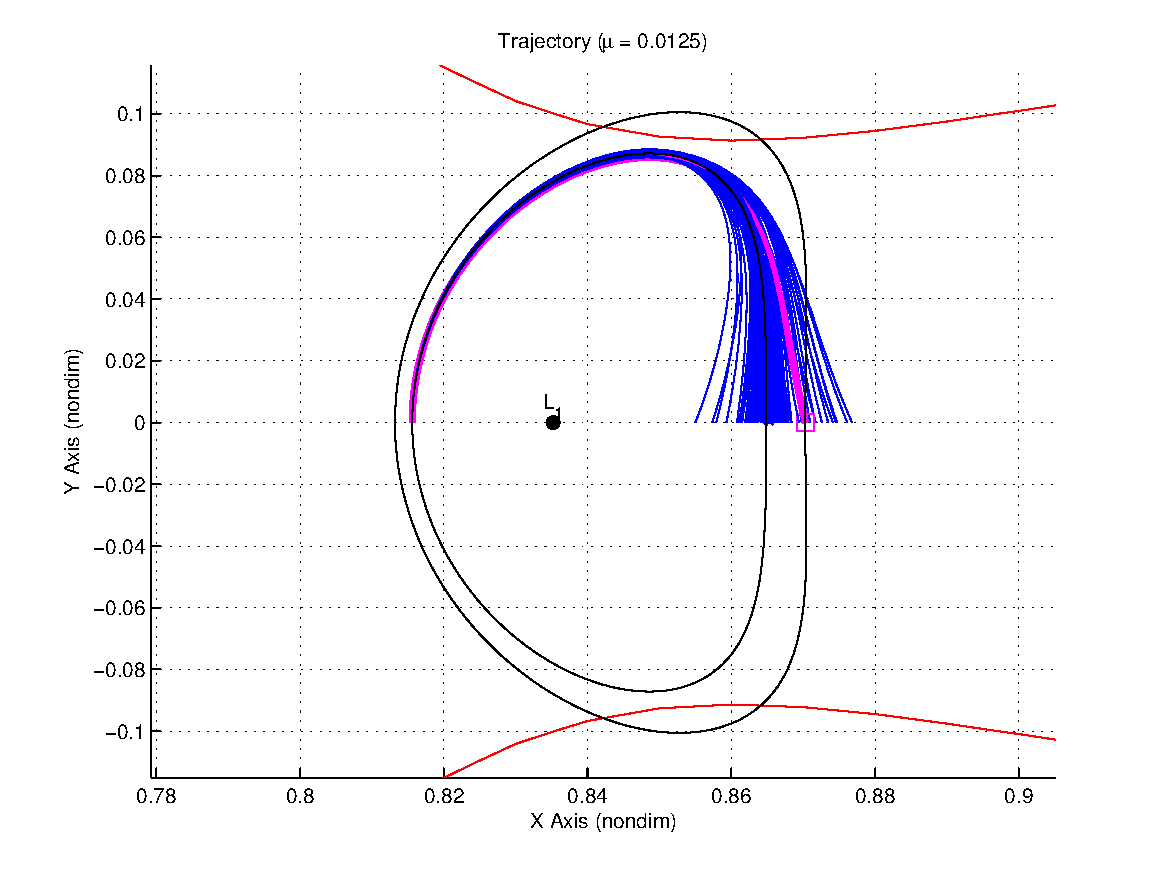
\includegraphics[width=\columnwidth]{figures/2015_SSPI/north_reach_trajectory}
        \caption{Trajectories}
        \label{fig:north_trajectory}
    \end{subfigure}
    ~
    \begin{subfigure}[b]{0.49\textwidth}
        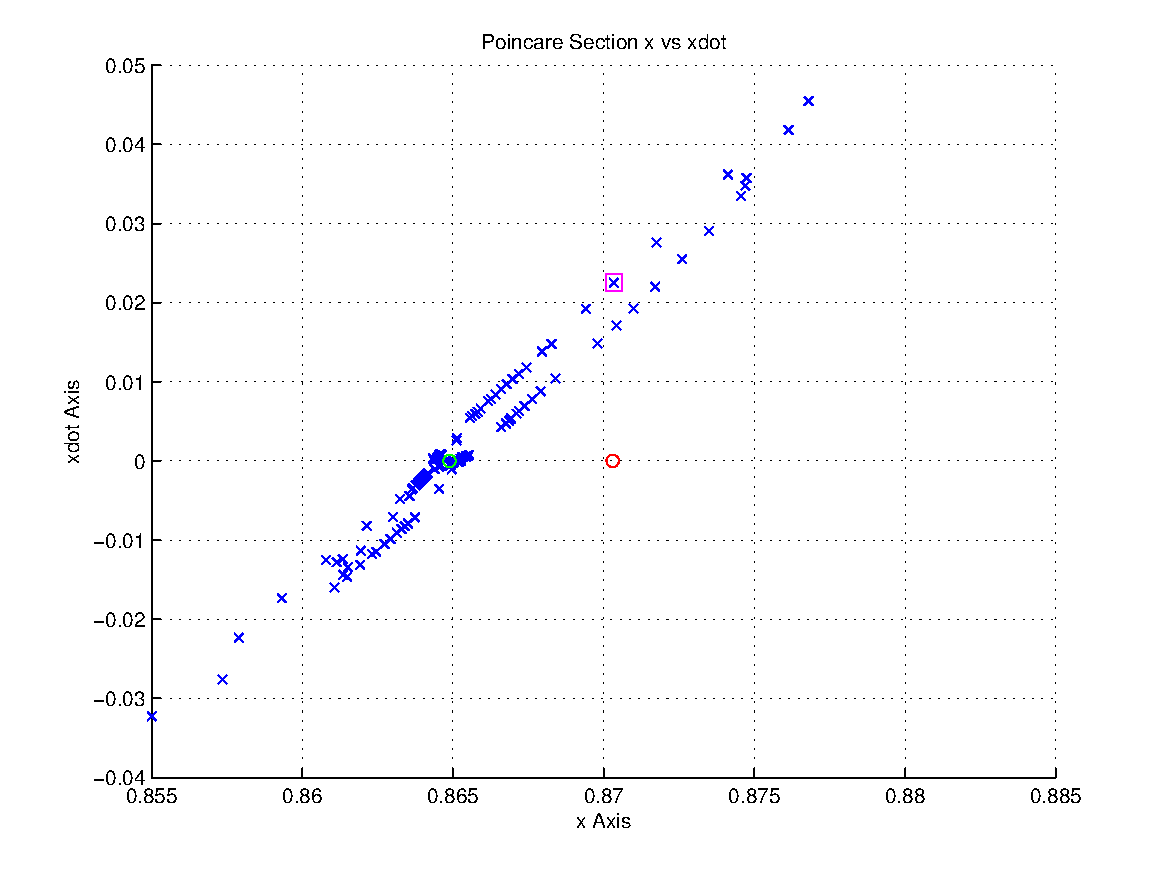
\includegraphics[width=\columnwidth]{figures/2015_SSPI/north_reach_poincare}
        \caption{Reachable set }
        \label{fig:north_poincare_reach}
    \end{subfigure}
    \caption{Northern Trajectories}\label{fig:north_reach}
\end{figure}
\begin{figure}[htbp]
        	\centering
        	\begin{subfigure}[b]{0.49\textwidth}
        		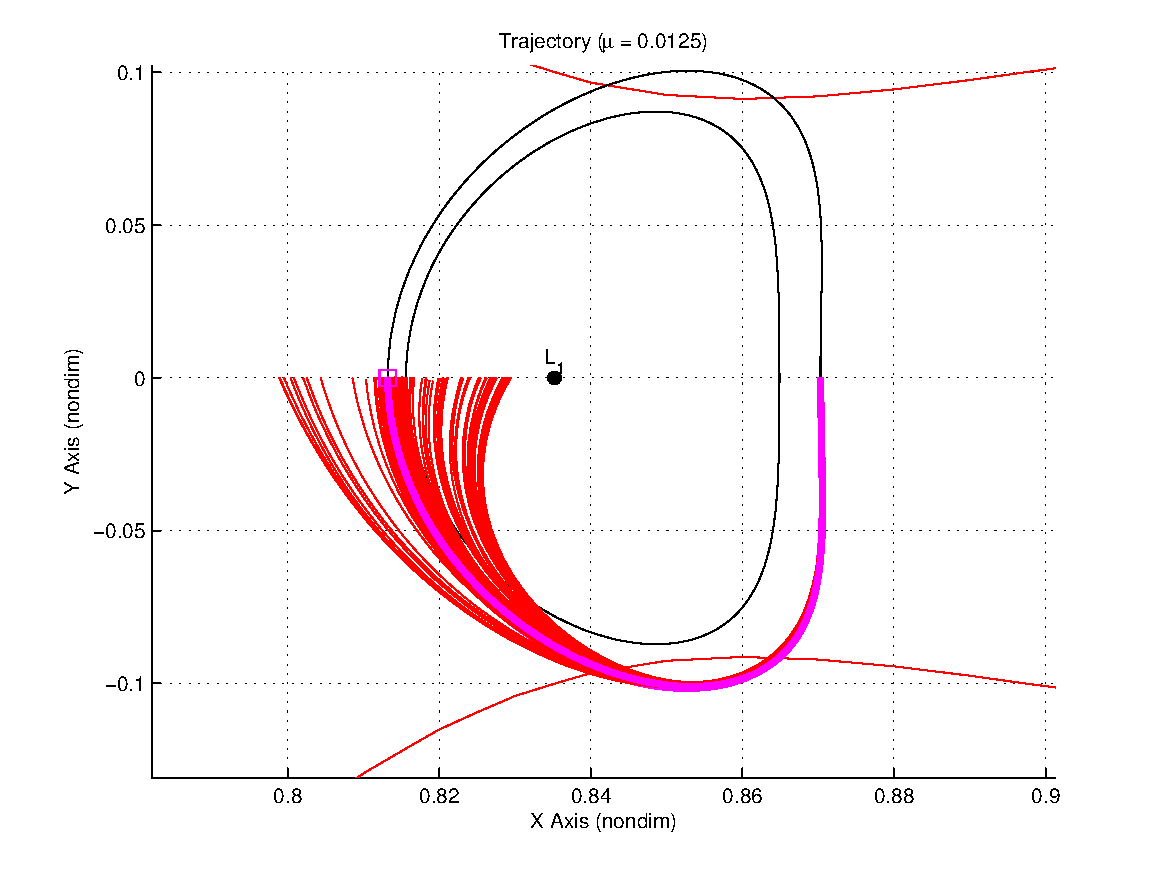
\includegraphics[width=\columnwidth]{figures/2015_SSPI/south_reach_trajectory}
        		\caption{Trajectories}
        		\label{fig:south_trajectory}
        	\end{subfigure}
			~
			\begin{subfigure}[b]{0.49\textwidth}
        		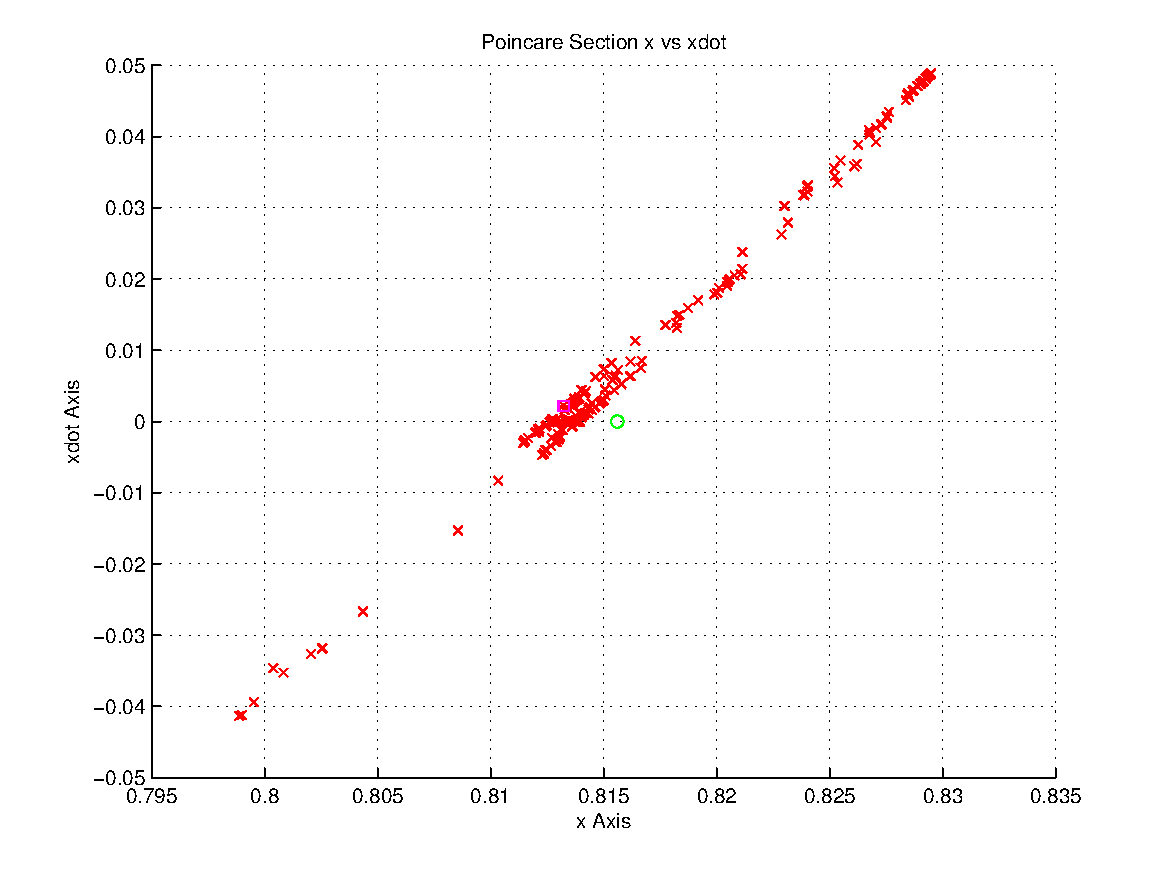
\includegraphics[width=\columnwidth]{figures/2015_SSPI/south_reach_poincare}
        		\caption{Reachable set }
        		\label{fig:south_poincare_reach}
        	\end{subfigure}
	\caption{Southern Trajectories}\label{fig:south_reach}
        \end{figure}	        
\begin{figure}[!htbp]
	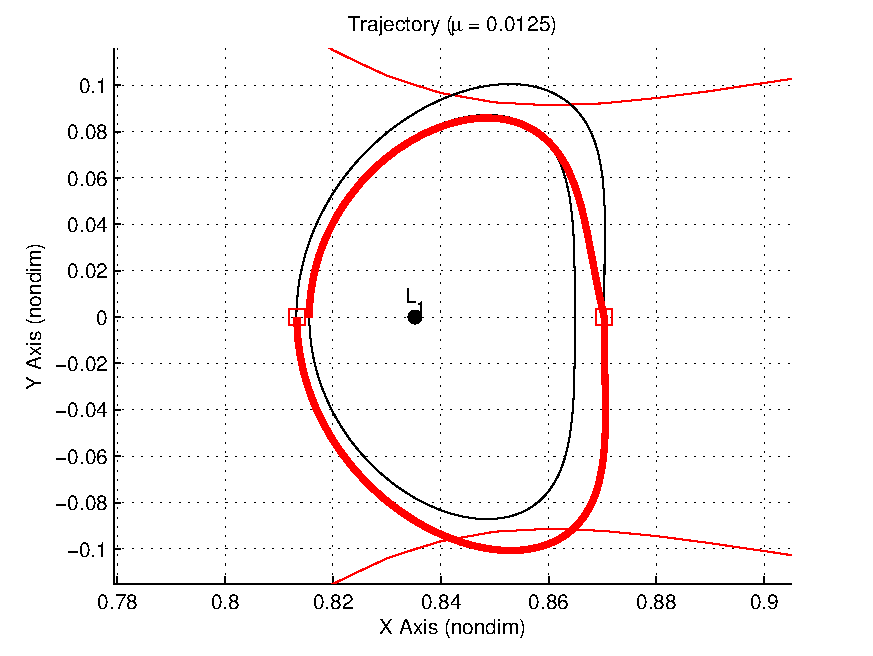
\includegraphics[width=0.5\textheight]{figures/2015_SSPI/opt_reach_trajectory}
	\caption{Optimal transfer trajectory}
	\label{fig:opt_reach_trajectory}
\end{figure}
\begin{figure}[!htbp]
	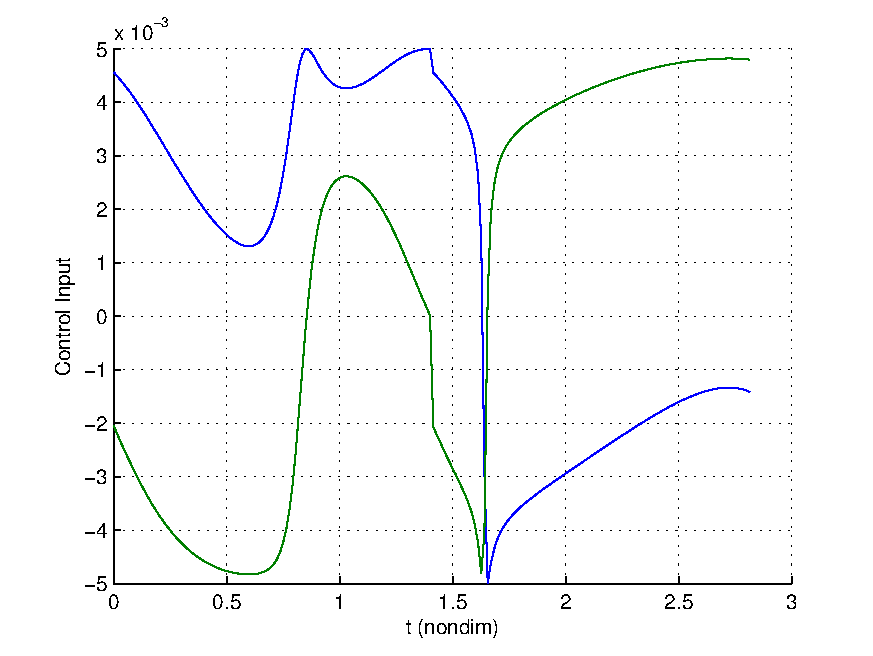
\includegraphics[width=0.5\textheight]{figures/2015_SSPI/opt_reach_control}
	\caption{Optimal control input}
	\label{fig:opt_reach_control}
\end{figure}
\section{Conclusion}
In this work an optimal transfer process which combines concepts of reachability and Poincar\'e section is used to generate transfer between planar periodic orbits in the three body problem.
The Poincar\'e section allows for trajectory design on a lower dimensional phase space and simplifies the process.
The indirect optimal control formulation enables straightforward method of incorporating additional path and control constraints.
However, the use of optimal control techniques leads to open loop trajectories that are not robust to model uncertainties or disturbances.
Lyapunov control theory, which has previously been applied to the two body problem~\cite{chang2002}, is being investigated in the hope of designing closed loop control schemes for this three-body scenario.
The current work is developed using continuous time equations of motion. 
When implemented within a computer system, these continuous time necessary conditions are discretized implicitly during simulation.
Future work will aim to develop a discrete time optimization problem using variational integrators. 
The discrete time formulation has been shown to provide significant advantages and energy conserving properties.

